The general equation of second degree can be expressed as
\begin{align}
	\vec{x}^{T}\vec{Vx} + 2\vec{u}^{T}\vec{x} + f=0   \label{eq:solutions/40/6/stdsecdeg}
\end{align}
where
\begin{align}
        \vec{V}=\vec{V}^T=\myvec{a & b \\ b & c}   \label{eq:solutions/40/6/V}  \\
        \vec{u}^T=\myvec{d &  e}            \label{eq:solutions/40/6/u}
\end{align}
From (\ref{eq:solutions/40/6/V}) and (\ref{eq:solutions/40/6/u})
\begin{align}
	\vec{V}=\vec{V}^T &= \myvec{3 & -4 \\ -4 & -3} \\
	\vec{u} &= \myvec{5 \\ -\frac{13}{2}}
\end{align}
\begin{align}
	\mydet{\vec{V}}=\mydet{3 & -4 \\ -4 & 3} =-25 \\
	\implies \mydet{\vec{V}} < 0       \label{eq:solutions/40/6/detless0}
\end{align}
Since $ \vec{V} = \vec{V}^T $, there exists an orthogonal matrix $\vec{P}$ such that
\begin{align}
	\vec{P}\vec{V}\vec{P}^T = \vec{D} = diag\myvec{\lambda_1 & \lambda_2}
\end{align}
or equivalently 
\begin{align}
	\vec{V} = \vec{P}\vec{D}\vec{P}^T
\end{align}
Eigen vectors of real symmetric matrix $\vec{V}$ are orthogonal. The characteristic equation of $\vec{V}$ is obtained by evaluating the determinant
\begin{align}
	\mydet{\lambda\vec{I}-\vec{V}} = \mydet{\lambda-3 & 4 \\ 4 & \lambda + 3} = 0 \\
	\implies \quad \lambda^2-25=0 \\
	\implies \quad \lambda_1=-5,\lambda_2=5   \label{eq:solutions/40/6/lambdavals}
\end{align}
From (\ref{eq:solutions/40/6/detless0}) and (\ref{eq:solutions/40/6/lambdavals}) the equation represents a hyperbola.
The eigen vector $\vec{p}$ is defined as
\begin{align}
	\vec{V}\vec{p}=\lambda\vec{p} \\
	\implies (\lambda\vec{I} - \vec{V})\vec{p}=0
\end{align}
For $\lambda_1 = -5$ :
\begin{align}
	(\lambda_1\vec{I}-\vec{V})=\myvec{-8 & 4 \\ 4 & -2} 
	\xleftrightarrow[R_2 \leftarrow \frac{R_2}{2}]{R_1 \leftarrow -\frac{R_1}{4}}
	\myvec{2 & -1 \\ 2 & -1} \\
	\xleftrightarrow[]{R_2 \leftarrow R_2 - R_1}
	\myvec{2 & -1 \\ 0 & 0} \\
	\implies \vec{p_1}=\frac{1}{\sqrt{5}}\myvec{2 \\ 1}
\end{align}
Similarly, the eigenvector corresponding to $\lambda_2$ can be obtained as
\begin{align}
	\vec{p_2}=\frac{1}{\sqrt{5}}\myvec{-1\\2}
\end{align}
The orthogonal eigen-vector matrix
\begin{align}
	\vec{P}=\myvec{\vec{p_1} & \vec{p_2}}
	=\frac{1}{\sqrt{5}}\myvec{2 & -1 \\ 1 & 2} \\
	\vec{D}=\myvec{-5 & 0 \\ 0 & 5}
\end{align}
Let $\vec{x}=\vec{P}\vec{y} + \vec{c} $ with $\vec{c}=-\vec{V}^{-1}\vec{u}$. Substituting in (\ref{eq:solutions/40/6/stdsecdeg})
\begin{align}
	\vec{y}^T\vec{D}\vec{y}=\vec{u}^T\vec{V}^{-1}\vec{u}-f 
\end{align}
with centre
\begin{align}
	\vec{c}=-\vec{V^{-1}u}=\myvec{-\frac{41}{25} \\ \frac{1}{50}} 
\end{align}
and minor and major axes parameters as
\begin{align}
	\sqrt{\frac{\lambda_1}{f-\vec{u^{T}V^{-1}u}}} = \sqrt{\frac{500}{33}}, \
	\sqrt{\frac{\lambda_2}{\vec{u^{T}V^{-1}u}-f}} = \sqrt{\frac{500}{33}}
\end{align}
The equation of hyperbola is
\begin{align}
	\frac{y_2^2}{\frac{33}{500}}-\frac{y_1^2}{\frac{33}{500}}=1
\end{align}
\begin{figure}[!h]
	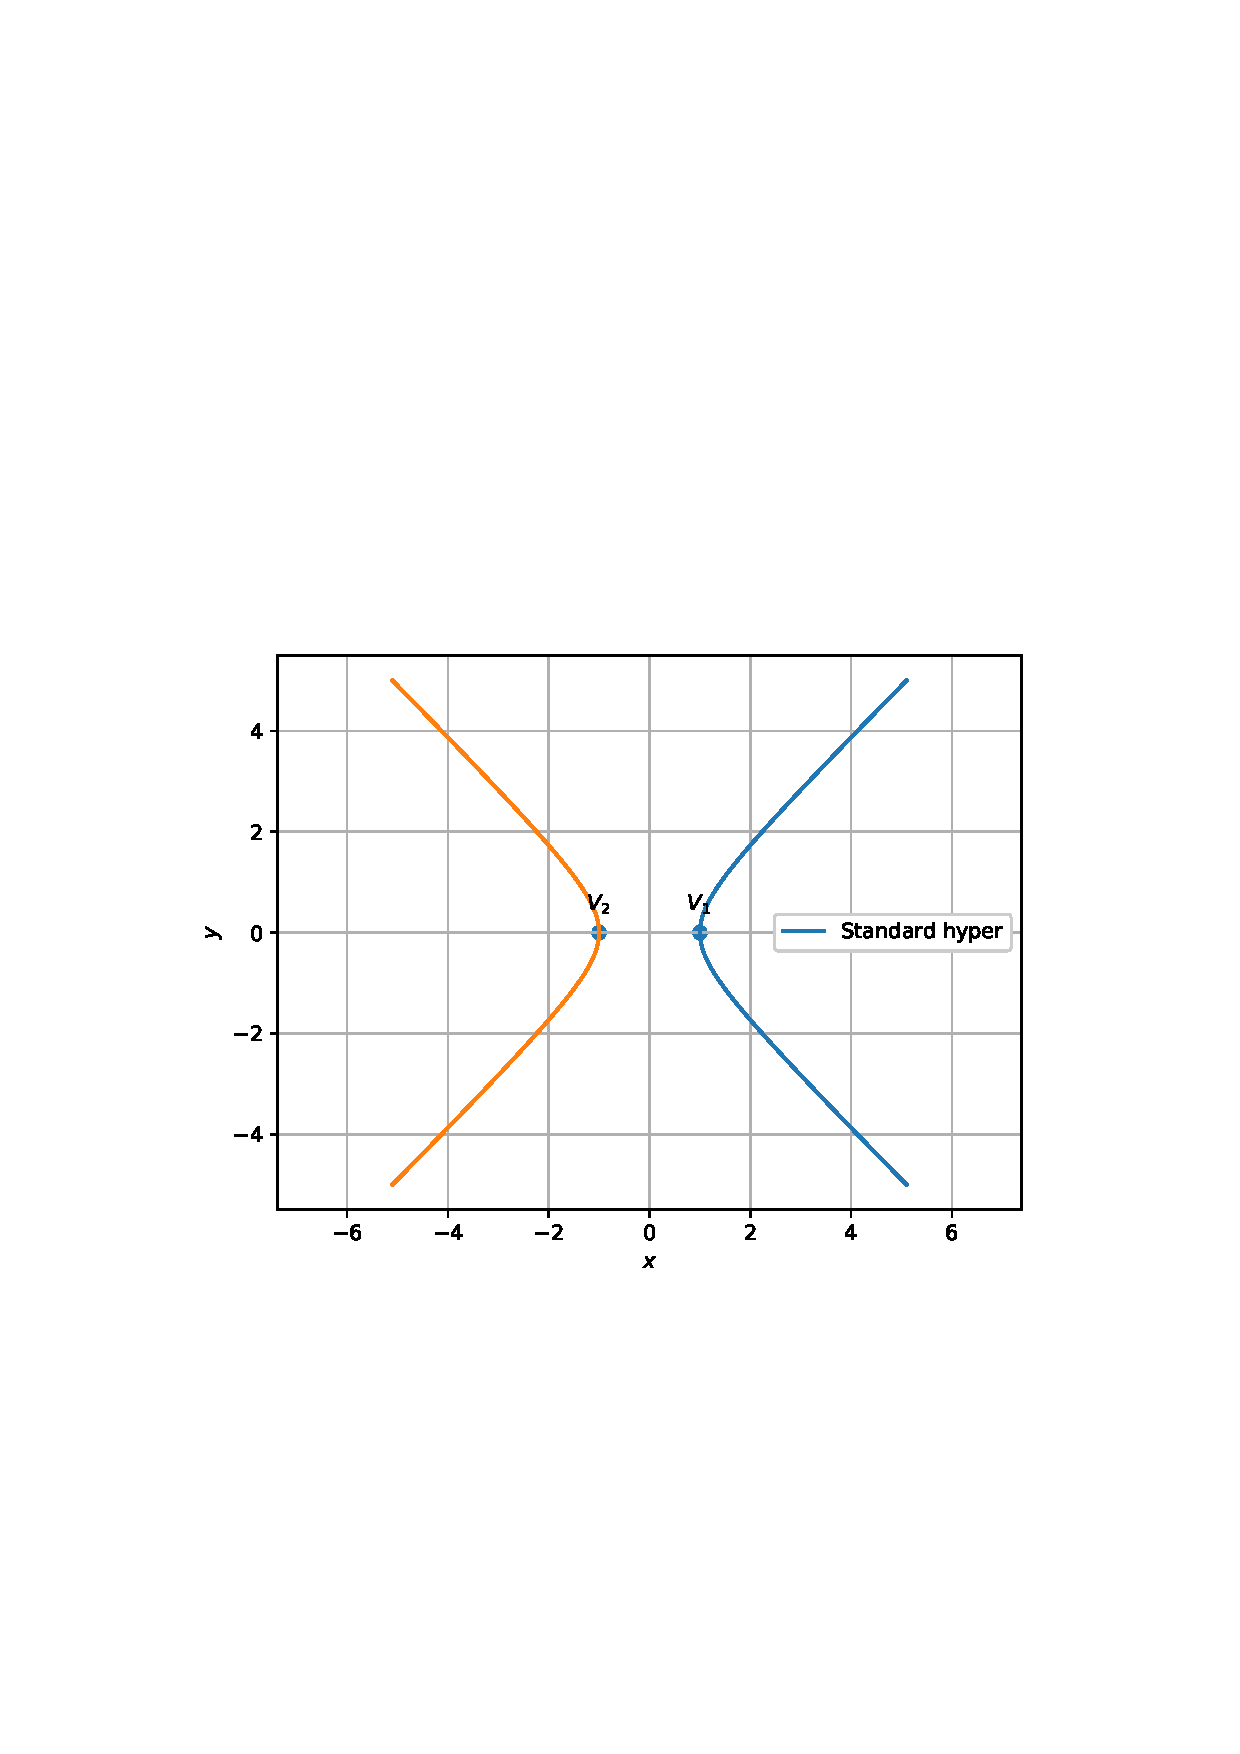
\includegraphics[width=\columnwidth]{./solutions/40/6/hyper.png}
	\caption{} \label{eq:solutions/40/6/linefig1}
\end{figure}
